% TODO: 
% -- load our code onto Matlab Central.
% % gs -sDEVICE=pdfwrite -dCompatibilityLevel=1.4 -dNOPAUSE -dQUIET -dBATCH      -sOutputFile=CompressedAssembly.pdf Assembly.pdf
\pdfobjcompresslevel=0  % I had adobe error 131, and this removed it: http://tex.stackexchange.com/questions/64448/how-to-overcome-acrobat-reader-error-131-with-a-pdflatex-doc
%\documentclass[letterpaper, 10 pt, conference]{ieeeconf}
\documentclass[letterpaper, 10 pt, journal, twoside]{ieeetran} 

% Paper headers 
\markboth{IEEE Robotics and Automation Letters. Preprint Version. Accepted May, 2017}
{Manzoor \MakeLowercase{\textit{et al.}}: Parallel Self-Assembly of Polyominoes under Uniform Control Inputs}  

\IEEEoverridecommandlockouts
\usepackage{calc}
\usepackage{url}
\usepackage{hyperref}
\usepackage[usenames, dvipsnames]{color}
\definecolor{darkblue}{rgb}{0,0,0.5}
\hypersetup{
  colorlinks =true,
  urlcolor = darkblue,
  linkcolor = darkblue,
  citecolor =darkblue
}
\usepackage{graphicx}
\usepackage[cmex10]{amsmath}
\usepackage{amssymb}
\usepackage{rotating}
\usepackage{booktabs}
\usepackage{rotating}
\usepackage{nicefrac}
\usepackage{cite}
\usepackage[caption=false,font=footnotesize]{subfig}
\usepackage{amsthm} % for proofs

\usepackage{colortbl}
\usepackage{overpic}
\graphicspath{{./pictures/pdf/},{./pictures/ps/},{./pictures/png/},{./pictures/jpg/}}
\usepackage{breqn} %for breaking equations automatically
\usepackage[ruled]{algorithm}
%\usepackage[noend]{algorithmic}
%\usepackage{algorithmicext}
%\usepackage{ifthen}
\usepackage{algpseudocode}
\algtext*{EndWhile}% Remove "end while" text
\algtext*{EndIf}% Remove "end if" text
\algtext*{EndFor}% Remove "end if" text
\usepackage{multirow}



\usepackage{bm}   % boldface math type
\usepackage{soul}  % for highlighting
\newcommand{\todo}[1]{\vspace{5 mm}\par \noindent \framebox{\begin{minipage}[c]{0.98 \columnwidth} \ttfamily\flushleft \textcolor{red}{#1}\end{minipage}}\vspace{5 mm}\par}
% uncomment this to hide all red todos
%\renewcommand{\todo}{}

%% ABBREVIATIONS
\newcommand{\figwid}{0.22\columnwidth}
\DeclareMathOperator{\atan2}{atan2}
\newtheorem{theorem}{Theorem}
\newtheorem{definition}[theorem]{Definition}
\newtheorem{lemma}[theorem]{Lemma}
\newtheorem{corollary}[theorem]{Corollary}







\begin{document}


\title{Parallel Self-Assembly of Polyominoes under Uniform Control Inputs}
\author{Sheryl Manzoor$^{1}$, Samuel Sheckman$^{2}$, Jarrett Lonsford$^{1}$, Hoyeon Kim$^{2}$, Min Jun Kim$^{2}$, and Aaron T. Becker$^{1}$% <-this % stops a space
\thanks{Manuscript received: Feb., 15, 2017; Revised May, 3, 2017; Accepted May, 26, 2017.}%Use only for final RAL version
\thanks{This paper was recommended for publication by Editor Yu Sun upon evaluation of the Associate Editor and Reviewers' comments. *This work was supported by the National Science Foundation under Grant No.\ \href{http://nsf.gov/awardsearch/showAward?AWD_ID=1553063}{ [IIS-1553063]}, \href{http://nsf.gov/awardsearch/showAward?AWD_ID=1619278}{[IIS-1619278]}, and \href{https://nsf.gov/awardsearch/showAward?AWD_ID=1712088}{[IIS-1712088]}.}%Use only for final RAL version
\thanks{$^{1}$S.~Manzoor, J Lonsford, and  A.~Becker are with the Department of Electrical and Computer Engineering,  University of Houston, Houston, TX 77204 USA        {\tt\small  \{smanzoor2, jllonsford, atbecker\}@uh.edu}}%
\thanks{$^{2} $S.~Sheckman, H.~Kim and M.J.~Kim are with Lyle School of Engineering,   Southern Methodist University, Dallas, TX 75205 USA        {\tt\small  \{ssheckman, hoyeonk, mjkim\}@smu.edu}}%
\thanks{Digital Object Identifier (DOI): see top of this page.}
}
\maketitle


\begin{abstract} 
We present fundamental progress on parallel self-assembly using large swarms of micro-scale particles in complex environments, controlled not by individual navigation, but by a uniform, global, external force with the same effect on each particle.
Consider a 2D grid world, in which all obstacles and particles are unit squares,
and for each actuation, robots move maximally until they collide with an obstacle or another robot. 
We present algorithms that, given an arbitrary 2D structure, design an obstacle layout.
 When actuated, this layout generates copies of the input 2D structure.
We analyze the movement and spatial complexity of the factory layouts. 
We present hardware results on both a macro-scale, gravity-based system and a micro-scale, magnetically-actuated system.
\end{abstract}
\begin{IEEEkeywords}
Automation at Micro-Nano Scales; Additive Manufacturing; Underactuated Robots
\end{IEEEkeywords}

%%% The paper
%###############################################################
\section{Introduction}\label{sec:Intro}
%###############################################################

One of the exciting new directions of robotics is the design and development
of micro- and nanorobot systems, with the goal of letting a massive swarm of robots
perform complex operations in a complicated environment. Due to scaling 
issues, individual control of the involved robots becomes physically impossible:
while energy storage capacity drops with the third power of robot size,
medium resistance decreases much slower. As a consequence,
current micro- and nanorobot systems with many robots are steered and
directed by an external force that acts as a common control signal~\cite{Donald2013,Chiang2011,Hsi-Wen2012,Diller2013,Jing2013,Ou2013,Lanauze2013}.
These common control signals include global magnetic or electric fields,
chemical gradients, and turning a light source on and off.  

 \subsection{Selective Control with Global Inputs}
Clearly, having only one global signal that uniformly affects all robots at once
poses a strong restriction on the ability of the swarm to perform complex operations.
This control symmetry can be broken using interactions between the robot swarm
and obstacles in the environment. The key challenge is to establish
if interactions with obstacles are sufficient to perform complex operations, ideally by analyzing the complexity of possible logical operations.
 In previous work \cite{Becker2013f,Becker2014,Becker2014a},
we were able to demonstrate how a subset of logical functions can be implemented;
however, devising a fan-out gate (and thus the ability to replicate and copy information)
appeared to be prohibitively challenging. In this paper, we resolve this crucial question by
showing that only using unit-sized robots is insufficient for achieving computational
universality. Remarkably, adding a limited number of domino-shaped objects {\em is sufficient}
to let a common control signal, mobile particles, and unit-sized obstacles
simulate a computer. While this does not imply that large-scale computational 
tasks should be run on these particle computers instead of current electronic
devices, it establishes that future nano-scale systems are able to perform
arbitrarily complex operations {\em as part of the physical system}, instead
of having to go through external computational devices.


%\begin{figure}
 %  \centering
%\begin{overpic}[width =\columnwidth]{7tilefactory.jpg}
%\end{overpic}
%\caption{\label{fig:7tilefactory}A seven tile factory.  Each particle is actuated simultaneously by the same global control field.  The factory (black tiles) is designed so each clockwise control input assembles another component.
%}
%\end{figure}

\begin{figure}

\centering
\subfloat[]{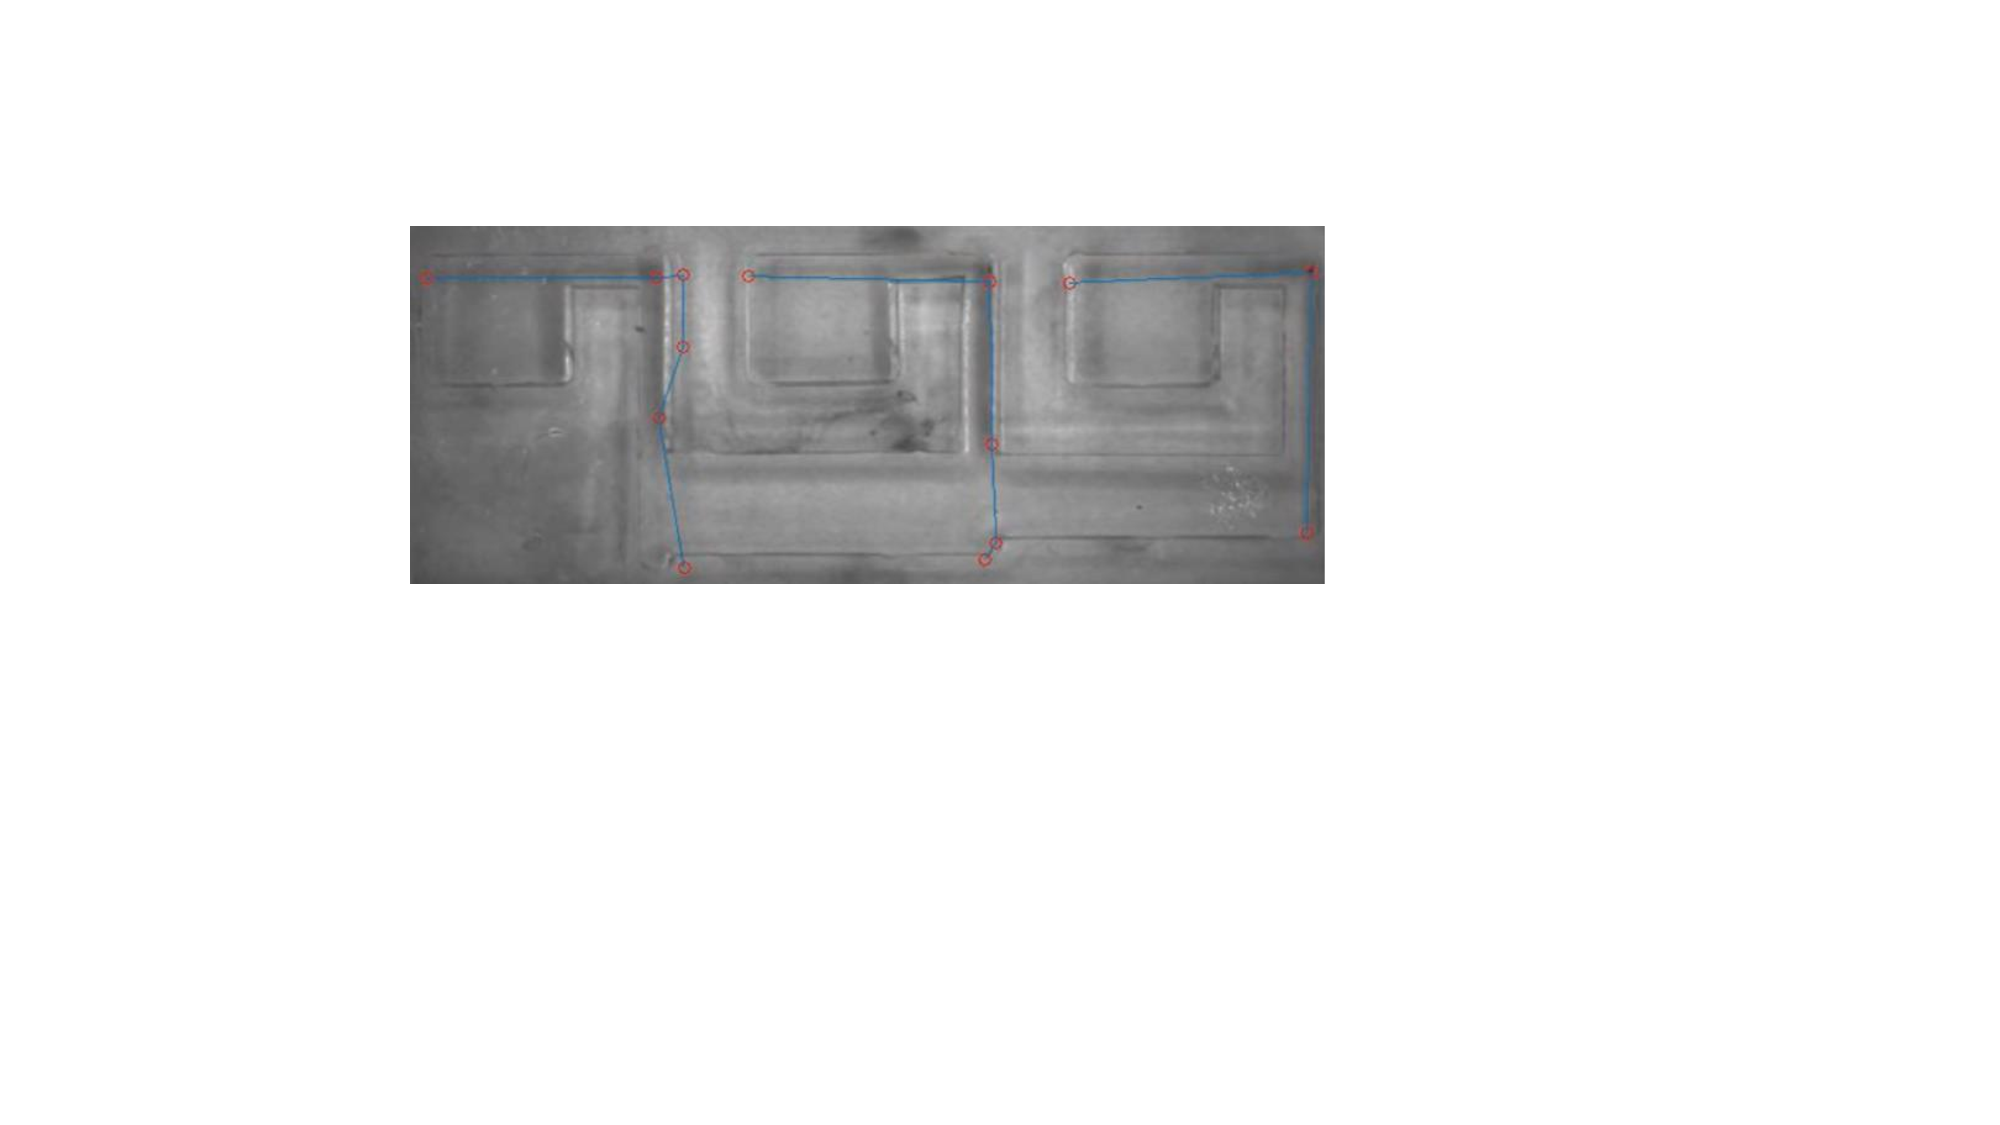
\includegraphics[width=3.1in]{fig1a.pdf}} 
\label{fig:fig1}
\newline
\subfloat[]{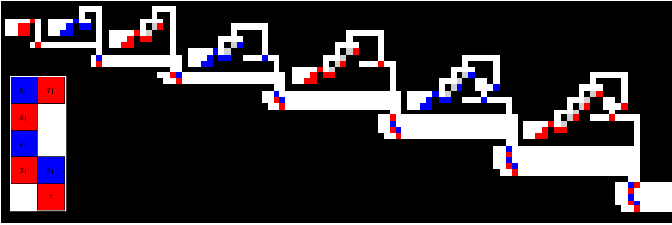
\includegraphics[width=3.1in]{fig1b1.pdf}}
\label{fig:fig2}
\caption{(a) A milli-scale magnetic based prototype.
 (b) A seven tile factory. Each particle is actuated simultaneously by the same global field. The factory is designed so each clockwise control input assembles another component.}
\label{fig:1} 

\end{figure}






%   \begin{figure}
%   \centering
%   \href{http://youtu.be/EJSv8ny31r8}{
%\begin{overpic}[width =\columnwidth]{DSC_0093lowres.JPG}%\put(30,-7){ $m=1$, partition 1}
%\end{overpic}}
%\caption{\label{fig:prototype}
%Gravity-fed hardware implementation of  particle computation.  The reconfigurable prototype is setup as a {\sc fan-out} gate using a 2$\times$1 robot (white). This paper proves that such a gate is impossible using only 1$\times$1 robots. \href{http://youtu.be/EJSv8ny31r8}{See the demonstrations in the video attachment \url{http://youtu.be/EJSv8ny31r8}.} }
%\vspace{-1em}
%\end{figure}

 \subsection{Model}
  
This paper builds on the techniques for controlling many simple robots with uniform control inputs presented in \cite{Becker2013f,Becker2014,Becker2014a}, using the following rules:
\begin{enumerate}
\item A planar  grid \emph{workspace} $W$ is filled with a number of unit-square robots (each occupying one cell of the grid)  and some fixed unit-square blocks.  Each unit square in the workspace is either  \emph{free}, which a robot may occupy or \emph{obstacle} which a robot may not occupy.  Each square in the grid can be referenced by its Cartesian coordinates $\bm{x}=(x,y)$.
\item All robots are commanded in unison: the valid commands are  ``Go Up" ($u$), ``Go Right" ($r$), ``Go Down" ($d$), or ``Go Left" ($l$).  
\item Robots all move in the commanded direction until they 
	\begin{enumerate}
		\item hit an obstacle 
		\item hit a stationary robot. 
		\item share an edge with a compatible robot
	\end{enumerate}
	If a robot shares an edge with a compatible robot the two robots bond and from then on move as a unit.
A \emph{move sequence} $\bm{m}$ consists of an ordered sequence of moves $m_k$, where each $m_k\in\{u,d,r,l\}$  A representative move sequence is $\langle u,r,d,l,d,r,u,\ldots\rangle$. We assume the area of $W$ is finite and issue each command long enough for the robots to reach their maximum extent.
\end{enumerate}

%###############################################################
\section{Related Work}\label{sec:RelatedWork}
%###############################################################


\subsection{Microscale Biomanufacturing}
Naturally derived biomaterials as building blocks for functional materials and devices are increasingly desired because they are environmentally and biologically safer than purely synthetic materials. One such class of materials, polysaccharide based hydrogels, are intriguing because they can reversibly encapsulate a variety of smaller components. Many groups have termed these loaded-alginate particles as artificial cells, in that they mimic the basic structure of living cells (membrane, cytoplasm, organelles, etc.) \cite{chang2005therapeutic} [1-3]. Construction with these micron-sized gels has numerous applications in industry, including cell manipulation, tissue engineering, and micro-particle assembly [4-8], but requires fundamental research in biology, medicine, and colloidal science. While there are several methods to efficiently fabricate these particulate systems, it is still challenging to construct larger composite materials out of these units [9]. Traditional methods of assembling larger macroscale systems are unemployable due to the change of dominant forces at small length scales. In particular, forces due to electromagnetic interactions dominate gravitational forces at the microscale resulting in strong adhesion and sudden shifts in the position of microparts under atmospheric conditions. Furthermore, analogs of basic macroscale robotic elements have not been suitably designed and commercialized. To form constructs out of microgels, groups have traditionally turned to non-robotic microfluidic systems that utilize a variety of actuation methods, including mechanical, optical, dielectrophoretic, acoustophoretic, and thermophoretic [10-14]. While each of these methods has proven to be capable of manipulating biological cells, each method has significant drawbacks that limit their widespread application. For example, microscale mechanical, acoustophoretic, and thermophoretic manipulation methods use stimuli that can be potentially lethal to live cells [15]. Furthermore, most, if not all, of these techniques require expensive equipment and lack control schemes necessary to precisely manipulate large numbers of cells autonomously.

\subsection{Control of Microrobotic Swarms Using Only Global Signals}
Today one of the most exciting new frontiers in robotics is the development of micro- and nanorobotic systems, which hold the potential to revolutionize the fields of manufacturing and medicine. Chemist, biologist, and roboticist have shown the ability to produce very large populations (103-1014) of small scale (10-9-10-6 m) robots using a diverse array of materials and techniques [16-18]. Untethered swarms of these tiny robots may be ideal for on-site construction of high-resolution macroscale materials and devices. While these new types of large-population, small-sized, robotic systems have many advantages over their larger-scale counterparts, they also present a set of unique challenges in terms of their control. Due to 

current limitations in fabrication, micro- and nanorobots have little-to-no onboard computation, along with limited computation and communication ability [18-20]. These limitations make controlling swarms of these robots individually impractical. Thus, these robotic systems are often controlled by a uniform global external signal (e.g. chemical gradients, electric and magnetic fields), which makes motion planning for large robotic populations in tortuous environments difficult. However, it was recently demonstrated that obstacles present in the workspace can break the symmetry of approximately identical robotic swarms, enabling positional configuration of robots [21]. Using this novel method, it was shown that, given a large-enough free space, a single obstacle is sufficient for positional control over N particles.  This method can be used to form complex assemblies out of large swarms of mobile microrobotic building blocks, using only a single global input signal.

\subsection{Microrobot Based Microassembly}
The ability to create microrobots, and control algorithms capable of autonomous manipulation and assembly of small scale components into functional materials is currently a major manufacturing challenge [1]. To address this challenge, teams of microrobotic systems must work together intelligently to coordinate manipulation tasks in novel environments. While several microrobots capable of performing simple manipulation and assembly tasks have been reported [2-7], few have shown the ability to pattern intricate designs or assemble complex multi-component parts. Recently, some groups have begun to develop cell-safe magnetically actuated microrobotic systems for cell patterning, yet their method is limited in that these systems are manually controlled, not automated, and suffer from low spatial resolution [22, 23]. In this project, we seek to combine the use of microscale hybrid organic/inorganic actuators along with novel swarm control algorithms for object manipulation, mask free programmable patterning, and micro-assembly. Specifically, we will apply swarm control and particle logic computations to magnetically actuate artificial cells, so as to use them as micro-scale robotic swarms, to create complex, high resolution, 2D and 3D patterns and assemblies.
%###############################################################
\section{Theory}\label{sec:Theory}
%###############################################################

This section explains how to design factories that build arbitrary-shaped 2D polyominoes.
 We first assign species to individual tiles of the polyomino, second discover a build path, and finally build an assembly line of factory components that each add one tile to a partially assembled polyomino and pass the polyomino to the next component.


%###############################################################
\subsection{Arbitrary 2D shapes require two particle species}\label{subsec:RobotSpecies}
%###############################################################
A \emph{polyomino} is a 2D geometric figure formed by joining one or more equal squares edge to edge. Polyominoes have four-point connectivity.


\begin{lemma}
  Any polyomino can be constructed using just two species
  \end{lemma}
\begin{proof} 
Label a grid with an alternating pattern like a checkerboard.  Any desired polyomino can be constructed on this checkerboard, and all joints are between dissimilar species.
  An example shape is shown in Fig.~\ref{fig:Grid}.
  \end{proof}

   \begin{figure}
   \centering
\begin{overpic}[width =.8\columnwidth]{Grid2.pdf}
\end{overpic}
\caption{\label{fig:Grid}Any polyomino can be constructed with two compatible robot species.  
}
\end{figure}

  
  The sufficiency of two species to construct any shape gives many options for implementation.  The two species could correspond to any gendered connection, 
including electric charge, ionic charge, magnetic polarity, or hook-and-loop type fasteners.




%###############################################################
\subsection{Complexity Handled in This Paper}\label{sec:ComplexityHandled}
%###############################################################

Different 2D part geometries are more difficult to construct than others.  Fig.~\ref{fig:IncreasingDifficulty} shows parts with increasing  complexity. 

   \begin{figure}
   \centering
\begin{overpic}[width =\columnwidth]{IncreasingDifficulty3.pdf}
\end{overpic}
\caption{\label{fig:IncreasingDifficulty}Polyomino parts. Difficulty increases from left to right. Parts 4 and 5 cannot be built by additive construction. 
}
\end{figure} 
Label the first particle in the assembly process the \emph{seed particle}. 
 Part 1 is shaped as a `\#' symbol.  Though it has an interior hole, any of the 16 particles could serve as the seed particle, and the shape could be constructed around it.  The second shape is a spiral, and must be constructed from the inside-out.  If the outer spiral was completed first, there would be no path to add particles to finish the interior because added particles would have to slide past compatible particles.  Increasing the number of species would not solve this problem, because there is a narrow passage through the spiral that forces incoming parts to slide past the edges of all the bonded particles.
The third shape is contains a loop, and the interior must be finished before the loop is closed.
Shape 4 is the combination of a left-handed and a right-handed spiral.
 This part cannot be assembled by adding one particle at a time, because each spiral must be constructed from the inside-out.  
 Instead, this part must be divided into sub-assemblies that are each constructed, and then combined.
 Shape 5 contains compound overhangs, and may be impossible to construct with additive manufacturing.
 The algorithms in this paper detect if the desired shape can be constructed one particle at a time.  
 If so, a build order is provided, and a factory layout is designed.


% A polyomino is said to be \emph{column convex} if each column has no holes. Similarly, a polyomino is said to be row convex if each row has no holes. A polyomino is said to be \emph{convex} if it is row and column convex.
%
%\begin{lemma}\label{lemma:convexonjectsCanbeConstructedAdditively}
%Any convex polyomino can be constructed by adding one particle at a time
%\end{lemma}
%\begin{proof}
%Select any pixel as the \emph{seed block}, or root node.  Perform a breadth-first search starting at the seed block, labelling each block in the order they are expanded.  Constructing the shape according to the ordering ensures that the polyomino is convex at every step of construction.
%\end{proof}

%The proof of \ref{lemma:convexonjectsCanbeConstructedAdditively} assumes the existence of fixtures for assembly.
%\todo{describe fixtures for adding one particle at a time}

%Some non-convex polynominos cannot be constructed one particle at a time, as illustrated in Fig. ~\ref{fig:IncreasingDifficulty}.    For instance, a polynomino consisting of a clockwise and a counterclockwise square spiral, joined at the ends with a gap of one unit between the spirals must be constructed by first assembling each spiral, and then combining the sub assemblies.




%###############################################################
\subsection{Discovering a Build Path}
%###############################################################

Given a polyomino, Alg.~\ref{alg:FindBuildPath} determines if the polyomino can be built by adding one component at a time.
 The  problem of determining a build order is difficult because there are $O(n!)$ possible build orders, and many of them may  violate the constraints given in Section \ref{subsec:model}.  
 Each new tile must have a straight-line path to its goal position in the polyomino that does not collide with any other particle, does not slide past an opposite species of tile, and terminates in a mating configuration with an opposite species tile.
However, as in many robotics problem, the inverse problem of deconstruction is easier than the forward problem of construction.  

\begin{algorithm}
\newcommand\algotext[1]{\end{algorithmic}#1\begin{algorithmic}[1]}
%\begin{algorithmic}[1]
%\scriptsize 
\caption{\sc {FindBuildPath}($\mathbf{P})$   \label{alg:FindBuildPath}}
$\mathbf{P}$ is the $x,y$ coordinates of a 4-connected polyomino. % that has at least a 1-tile empty border.
Returns $ \mathbf{C} $, $ \mathbf{c} $ and $\mathbf{m}$ where $ \mathbf{C} $ contains sequence of polyomino coordinates, $ \mathbf{c} $ is a vector of color labels, and $\mathbf{m}$ is a vector of directions for assembly.
\begin{algorithmic}[1]

\State\hbox{$ \mathbf{c}\leftarrow${\sc{LabelColor}}($\mathbf{P}$)}
\State $\{\mathbf{C},\mathbf{m} \}= ${\sc {Decompose}}$(\mathbf{P},\mathbf{c})$
\State \Return $\{ \mathbf{C},\mathbf{c}, \mathbf{m} \} $ 
\end{algorithmic}
\end{algorithm} 

   \begin{figure}
   \centering
\begin{overpic}[width =\columnwidth]{DeconstructionOrderMattersSlide.pdf}
\end{overpic}
\caption{\label{fig:DeconstructionOrderMatters} Deconstruction order matters if loops are present.  Loops occur when the 8-connected freespace has more than one connected component.  In the top row, the green tile is removed first, resulting in a polyomino that cannot be decomposed. However, if the bottom right tile is removed first, deconstruction is possible.
}
\end{figure} 

Alg.~\ref{alg:FindBuildPath}  first assigns each tile in the polynomial a color, then calls the recursive function {\sc {Decompose}}, which returns either a build order of polyomino coordinates and the directions to build, or an empty list if the part cannot be constructed.  
{\sc {Decompose}} starts by calls the function {\sc {Erode}}.  {\sc {Erode}} first counts the number of components in the 8-connected freespace.  If there is more than one connected component, the polynomial contains loops.  
 {\sc {Erode}} maintains an array of the remaining tiles in the polyomino $\mathbf{R}$. 
 In the inner for loop at line  \ref{alg:line:forloopTotryremovinEachTileERODE}, a temporary array $\mathbf{T}$ is generated that contains all but the $j$th tile in $\mathbf{R}$.
This for loop simply checks (1) if the $j$th tile can be removed along a straight-line path without  colliding with any other particle or sliding past an opposite species of tile in line \ref{alg:line:checkpathtileERODE},  (2) that its removal does not fragment the remaining polyomino into more than one piece in line \ref{alg:line:NumConnectedCompERODE}, and (3) that its removal does not break a loop in line \ref{alg:line:Num8ConnectedCompERODE}. 
If no loops are present, this algorithm requires at most  $1/2 n (1 + n)$ iterations, because there are $n$ particles to remove, and each iteration considers one less particle than the previous iteration.

Polynomials with loops require care, because decomposing them in the wrong order can make disassembly impossible, as shown in Fig.~\ref{fig:DeconstructionOrderMatters}.
If loops exist then  {\sc {Erode}} may return only a partial decomposition, so {\sc {Decompose}} must then try every possible break point and recursively call {\sc {Decompose}} until either a solution is found, or all possible decomposition orders have been tested.  The worst-case number of function calls of  {\sc {Decompose}}  are proportional to the factorial of the number of loops, $O( |\text{\sc 8-ConnComp}(\neg\mathbf{P})| !)$. Though large, this is much less than $O(n!)$.

\begin{algorithm}
\newcommand\algotext[1]{\end{algorithmic}#1\begin{algorithmic}[1]}
%\scriptsize 
\caption{\sc {Erode}($\mathbf{P},\mathbf{c})$   \label{alg:Erode}}
$\mathbf{P}$ is the $x,y$ coordinates of a 4-connected polyomino  and $ \mathbf{c} $ is a vector of color labels.
Returns $ \mathbf{R} $, $ \mathbf{C} $, $\mathbf{m}$, and $\mathbf{\ell}$ where $ \mathbf{R} $  is a list of coordinates of the remaining polyomino, $ \mathbf{C} $ contains sequence of tile coordinates that were removed,   $\mathbf{m}$ is a vector of directions for assembly, and $\mathbf{\ell}$ if loops were encountered.
\begin{algorithmic}[1]

\State\hbox{$\mathbf{C} \leftarrow \{\}, \mathbf{m} \leftarrow \{\}, \mathbf{\ell} \gets \textrm{\sc False}$}
\State $\mathbf{d} \gets\{u,d,l,r\}, \mathbf{R} \gets \mathbf{P}$
\State $w \gets |\text{\sc 8-ConnComp}(\neg\mathbf{R})|$ 
\For{$i\leftarrow 1, i <  |\mathbf{P}| $}
\State  \emph{successRemove} $\gets$ {\sc False}
\For{$j\leftarrow 1, j \le  |\mathbf{R}| $}
\State $\mathbf{p} \gets \mathbf{R}_j,  \mathbf{T} \gets  \mathbf{R}  \backslash   \mathbf{R}_j$

\For{$ k \leftarrow 1, k \le  4$   \label{alg:line:forloopTotryremovinEachTileERODE} }
\If{{\sc CheckPathTile}($\mathbf{T},\mathbf{p}, \mathbf{d}_k, \mathbf{c}$) \label{alg:line:checkpathtileERODE} \textbf{and}
\\ \textbf{~~~~~~~~~~~~~~}
$1 = |\text{\sc 4-ConnComp}(\mathbf{T})|$  \label{alg:line:NumConnectedCompERODE}}
\If{$w = |\text{\sc 8-ConnComp}(\neg\mathbf{T})|$  \label{alg:line:Num8ConnectedCompERODE}}

\State  $\mathbf{R} \gets \mathbf{T}$,   \emph{successRemove} $\gets$ {\sc True}
\State  $\mathbf{C}_{ 1+|\mathbf{R}|} \gets \mathbf{p},  \mathbf{m}_{ |\mathbf{R}|}  \gets \mathbf{d}_k$
\Else { $  \mathbf{\ell} \gets \textrm{\sc True}$}
\EndIf
\State \textbf{break}
\EndIf
\EndFor
\EndFor
\If {  \emph{successRemove} $=$ {\sc False}}
\State  \hbox{$\mathbf{C} \leftarrow \{\}, \mathbf{m} \leftarrow \{\}$}
\State \textbf{break}
\EndIf
\EndFor
\If {$ |\mathbf{R}| = 1$}
\State  $\mathbf{C}_{ 1} \gets \mathbf{R}_1 $
\EndIf
\State \Return $\{ \mathbf{R},\mathbf{C}, \mathbf{m}, \ell \}$ 
\end{algorithmic}
\end{algorithm} 









\begin{algorithm}
\newcommand\algotext[1]{\end{algorithmic}#1\begin{algorithmic}[1]}
%\scriptsize 
\caption{\sc {Decompose}($\mathbf{P},\mathbf{c})$   \label{alg:Decompose}}
$\mathbf{P}$ is the $x,y$ coordinates of a 4-connected polyomino and $ \mathbf{c} $ is a vector of color labels.
Returns $ \mathbf{C} $ and $\mathbf{m}$ where $ \mathbf{C} $ contains sequence of polyomino coordinates and $\mathbf{m}$ is a vector of directions for assembly.
\begin{algorithmic}[1]

\State $ \{ \mathbf{R},\mathbf{C}, \mathbf{m}, \ell \} \gets ${\sc {Erode}}$(\mathbf{P},\mathbf{c})$
\If {$|  \mathbf{R} | = 0 \textbf{ or } \neg \ell$}
\State \Return $\{ \mathbf{C},\mathbf{m} \}$ 
\EndIf

\State $\mathbf{d} \gets\{u,d,l,r\}, \mathbf{R} \gets \mathbf{P}$
\For{$j\leftarrow 1, j \le  |\mathbf{R}| $}
\State $\mathbf{p} \gets \mathbf{R}_j,  \mathbf{T} \gets  \mathbf{R}  \backslash   \mathbf{R}_j$

\For{$ k \leftarrow 1, k \le  4$   \label{alg:line:forloopTotryremovinEachTileDecompose} }
\If{{ ( \sc CheckPathTile}($\mathbf{T},\mathbf{p}, \mathbf{d}_k, \mathbf{c}$) \label{alg:line:checkpathtileDecompose} \textbf{and }
\\ \textbf{~~~~~~~~~~~~ }
$1 = |\text{\sc 4-ConnComp}(\mathbf{T})|$)  \label{alg:line:NumConnectedCompDecompose}}
\State $\{\mathbf{C2},\mathbf{m2} \}\gets ${\sc {Decompose}}$(\mathbf{T},\mathbf{c})$
\If {$\mathbf{C2}  \ne \{\}$}
%\State  $\mathbf{C}_{ 1+|\mathbf{R}|} \gets \mathbf{p},  \mathbf{m}_{ |\mathbf{R}|}  \gets \mathbf{d}_k$
\State $\mathbf{C}_{1:|\mathbf{C2}|+1} \gets \{\mathbf{C2},\mathbf{p}\}$
\State $ \mathbf{m}_{1:|\mathbf{m2}|+1} \gets \{\mathbf{m2},\mathbf{d}_k\}$
\State \Return $\{ \mathbf{C}, \mathbf{m} \}$ 
\EndIf
\State \textbf{break}
\EndIf
%\EndIf
\EndFor
\EndFor
\State $\mathbf{C} \gets \{\}, \mathbf{m} \gets \{\}$
\State \Return $\{ \mathbf{C}, \mathbf{m} \}$ 
\end{algorithmic}
\end{algorithm} 



%\begin{algorithm}
%\newcommand\algotext[1]{\end{algorithmic}#1\begin{algorithmic}[1]}
%%\scriptsize 
%\caption{\sc {FindBuildPath}($\mathbf{P})$   \label{alg:FindBuildPath}}
%$\mathbf{P}$ is the $x,y$ coordinates of a 4-connected polyomino. 
%Returns $ \mathbf{C} $, $ \mathbf{c} $ and $\mathbf{m}$ where $ \mathbf{C} $ contains sequence of polyomino coordinates, $ \mathbf{c} $ is a vector of color labels and $\mathbf{m}$ is a vector of directions for assembly.
%\begin{algorithmic}[1]
%%\State$\mathbf{C} \leftarrow \{\}$,\State$ \mathbf{c} \leftarrow \{\}$, \State$ \mathbf{m} \leftarrow \{\}$
%\State\hbox{$\mathbf{C} \leftarrow \{\},\mathbf{c} \leftarrow \{\}, \mathbf{m} \leftarrow \{\}$}
%\State$\mathbf{c}\leftarrow${\sc{LabelColor}}($\mathbf{P}$)
%\For{$m\leftarrow 1, m \le  |\mathbf{P}| )$}
%\State$\mathbf{C}\leftarrow${\sc{DepthFirstSearch}}($\mathbf{P}_m$,$\mathbf{P}$)
%\State$ \mathbf{m}\leftarrow${\sc{CheckPathTile}}($\mathbf{C}$, $\mathbf{c}$)
%\If{$ \{\} \ne \mathbf{m}$}
%\State \textbf{break}
%\EndIf
%\EndFor\\
%\Return $\{ \mathbf{C},\mathbf{c}, \mathbf{m} \}$ 
%\end{algorithmic}
%\end{algorithm} 
  
%###############################################################
\subsection{Assembling Tiles}
%###############################################################


%###############################################################
\subsubsection{Hopper Construction}\label{subsec:HopperConstruction}
%###############################################################
Two-part adhesives react when the components mix.  Placing the components in separate containers prevents mixing.  Similarly, storing many particles of a single species in separate containers allows controlled mixing.
%WIKI: harden by mixing two or more components which chemically react.

We can design \emph{part hoppers}, containers that store similarly labelled particles.  These particles will not bond with each other.  The hopper shown in Fig.~\ref{fig:HopperCW} releases one particle every cycle. Delay blocks are used to ensure the $n$th part hopper does not start releasing particles until cycle $n$.

   \begin{figure}
   \centering
\begin{overpic}[width =\columnwidth]{hopperdirections.pdf}
\end{overpic}
\caption{\label{fig:HopperCW}Hopper with delays. The hopper is filled with similarly-labelled robots that will not combine.  Every clockwise command sequence $\langle u,r,d,l \rangle$ releases one robot from the hopper.  %\textcolor{red}{replace with new hopper design}
}
\end{figure}





\begin{figure}
   \centering
\begin{overpic}[width =\columnwidth]{24tilefactory.pdf}
\end{overpic}
\caption{\label{fig:24tilefactory}A twenty-four tile factory (full resolution -- zoom in for details).
}
\end{figure}







%###############################################################
\subsection{Part Assembly Jigs}\label{subsec:PartAssemblyJigs}
%###############################################################

Assembly is an iterative procedure.  
A factory layout is generated by  {\sc{BuildFactory}}($\mathbf{P}, n_c$), described in Alg.~\ref{alg:BuildFactory}. This function takes a 2D polyomino $\mathbf{P}$ and, if $\mathbf{P}$ has a valid build path, designs an obstacle layout to generate $n_c$ copies of the polyomino. A polyomino is composed of $|\mathbf{P}| = n$ tiles.  

For each tile, the function 
 {\sc{FactoryAddTile}} $(n_c,\mathbf{b}, m,C, c,w)$
  described in  Alg.~\ref{alg:FactoryAddTile}
is called to generate an obstacle configuration $\mathbf{A}$.
$\mathbf{A}$  forms a hopper that releases a particle each iteration and a chamber that temporarily holds the partially-assembled polyomino $\mathbf{b}$ and guides the new particle $C$ to the correct mating position. A 24-tile factory is shown in  Fig.~\ref{fig:24tilefactory}.


%\todo{Sheryl, add the algorithmic environment for Build Factory}
\begin{algorithm} 
\newcommand\algotext[1]{\end{algorithmic}#1\begin{algorithmic}[1]}
%\scriptsize
\caption{ \sc{BuildFactory}($\mathbf{P}, n_c$)\label{alg:BuildFactory}}
$\mathbf{P}$ is the $x,y$ coordinates of a 4-connected polyomino.  $n_c$ is the number of parts desired. 
Returns a two dimensional array $ \mathbf{F} $ containing the factory obstacles and filled hoppers.
\begin{algorithmic}[1]
\State$\mathbf{F} \leftarrow \{\}$ \Comment{the factory obstacle array} 
\State$ \mathbf{b} \leftarrow \{\}$ \Comment{the part being built} 

\State \{$\mathbf{C},\mathbf{c}, \mathbf{m}$\} $  \leftarrow$ {\sc{FindBuildPath}}($\mathbf{P}$)
 \If{$ \{\} = \mathbf{m}$}
 \State \Return  $ \mathbf{F} $
 \EndIf 
 \State$\{ \mathbf{A}, \mathbf{b} \}\leftarrow${\sc{FactoryFirstTile}}$(n_c, \mathbf{c}_i,w)$
 \For{$i\leftarrow 2, i \le  |\mathbf{c}| )$}
 \State$\{\mathbf{A},\mathbf{b}\}\leftarrow${\sc{FactoryAddTile}}$(n_c,\mathbf{b}, \mathbf{m}_{i-1},\mathbf{C}_i, \mathbf{c}_i,w)$
 \State$ \mathbf{F} \leftarrow${\sc{ConcatFactories}}$(\mathbf{F},\mathbf{A})$
\EndFor
\State \Return  $ \mathbf{F} $
%\State{\sc{DisplayFactory}}($factoryLayout$)
\end{algorithmic}
\end{algorithm} 
 
 
 

 
 
\begin{algorithm} 
\newcommand\algotext[1]{\end{algorithmic}#1\begin{algorithmic}[1]}
%\scriptsize
\caption{\sc {FactoryAddTile}$(n_c,\mathbf{b}, m,C, c,w)$ \label{alg:FactoryAddTile}}
\begin{algorithmic}[1]
\State$
\{ \mathbf{hopper}\}\leftarrow${\sc{Hopper}}$(c,n_c,w)$
\If{ $m = d \textbf{ and } \left(     C_x  \le \max \mathbf{b}_x   
                         \textbf{ or }  C_y     < \min \mathbf{b}_y \right)  }$
    
\State$\{\mathbf{A},\mathbf{b}\}\leftarrow${\sc{downdir}}$(\mathbf{hopper},\mathbf{b},\mathbf{C})$

\ElsIf{ $m = l \textbf{ and} \left(     C_y  \le \max \mathbf{b}_y   
                         \textbf{ or }  C_x     > \max \mathbf{b}_x \right)  }$
    
\State$\{\mathbf{A},\mathbf{b}\}\leftarrow${\sc{leftdir}}$(\mathbf{hopper},\mathbf{b},\mathbf{C})$
\ElsIf{ $m = l \textbf{ and} \left(     C_x  \ge \max \mathbf{b}_x   
                         \textbf{ or }  C_y     > \max \mathbf{b}_y \right)  }$
    
\State$\{\mathbf{A},\mathbf{b}\}\leftarrow${\sc{updir}}$(\mathbf{hopper},\mathbf{b},\mathbf{C})$
\ElsIf{ $m = r \textbf{ and } \left(     C_y     \ge \min \mathbf{b}_y   
                       \textbf{ or }  C_x  < \min \mathbf{b}_x   \right)  }$
\State$\{\mathbf{A},\mathbf{b}\}\leftarrow${\sc{rightdir}}$(\mathbf{hopper},\mathbf{b},\mathbf{C})$



\EndIf

\State \Return $\{ \mathbf{A}, \mathbf{b} \}$ 

\end{algorithmic}
\end{algorithm}
 
 
 
 
 
 






%###############################################################
\section{Analysis}\label{sec:Analysis}
%###############################################################
This section analyzes the time and space required for a factory and gives simulation results.


%###############################################################
\subsection{Running Time}\label{sec:runningTime}
%###############################################################
Running a factory simulation has three phases, ramp up, production, and wind down.
During the $n-1$ \emph{ramp up}  cycles, the first polyomino is being constructed one tile at a time and no polyominos are produced.
Clever design of delays in the part hoppers ensures no unconnected tiles are released.
During \emph{production} cycles, one  polyomino is finished each cycle.
Once the first part hopper empties, the $m-1$ \emph{wind down}  cycles each produce a complete polynomino as successive hoppers also empty.
 This section analyzes running time, defined as the time required for each commanded move until all tiles are stopped.  
 We assume all tiles move unit distance in unit time.
 There are two results, the \emph{construction time}, the time required to assemble a single polynomino from scratch, and
 the \emph{cycle time}, the time required during production cycles to advance all partial assemblies one cycle.
 Since a polyomino contains $n$ tiles, the \emph{construction time} during production cycles is $n \cdot$ \emph{cycle time}.
 
Cycle time is the sum of the maximum distances moved in each direction.
 As shown in Fig.~\ref{fig:timeplot}, polyominos shaped as a $n\times 1$ row require the longest time of $4n+16$.
Polyominos shaped as a $1\times n$ column require the least time of $2n+16$.
 Construction time therefore requires $O(n^2)$ time.
 \begin{figure}
   \centering
\begin{overpic}[width =1\columnwidth]{maxcycleplot.pdf}
\end{overpic}
\caption{\label{fig:timeplot}Cycle time plotted against number of tiles $n$.  The cycle time is the sum time to move in the $r,d,l,u$ moves each cycle. Cycle time increases linearly and is upper bounded by row parts and lower bounded by column parts.  Total construction time for a particle is $n \cdot $ cycle time.  
}
\end{figure}


%###############################################################
\subsection{Space Required}\label{sec:requiredSpace}
%###############################################################
The space required by a factory is a function of the size of individual sub-assemblies.

<<<<<<< HEAD
 \todo{tell us the big-Oh for  \emph{r} $\cdot$ \emph{c}.  Is it $n^2$ or $n^3$?}
 


$$
height(n)=
\begin{cases}
\left \lceil{nc/w}\right \rceil+2((\left \lceil{n/2}\right \rceil+1)+(partrows+1))    , 
& \text{for m=l or d}\\
\left \lceil{nc/w}\right \rceil+2((\left \lceil{n/2}\right \rceil+1)+(partrows+2))    , 
& \text{for m=l or d}

\end{cases}
$$
=======
Because a factory requires $O(n)$ rows and $O(n)$ columns, the total requires space is $O(n^2)$.
As shown in Fig.~\ref{fig:sizeplot}, the required size is  upper bounded by column-shaped polynominos and lower bounded by row-shaped polyominos, and is $O(n^2)$.

\begin{figure}
   \centering
\begin{overpic}[width =1\columnwidth]{facsizeplot1.pdf}
\end{overpic}
\caption{\label{fig:sizeplot}
Factory size grows quadratically with the number of tiles, and is upper bounded by column-shaped polynominos and lower bounded by row-shaped polyominos.
}
\end{figure}
>>>>>>> origin/master


%###############################################################
\subsection{Simulation Results}\label{sec:simResults}
%###############################################################

Algorithms  \ref{alg:FindBuildPath} through \ref{alg:FactoryAddTile}  were coded in {\sc Matlab} and are available at \cite{Manzoor2017gitAssemply}.  









%###############################################################
\section{Experiment}\label{sec:Experiment}
%###############################################################
To demonstrate  Algs.~\ref{alg:FindBuildPath}--\ref{alg:FactoryAddTile}, we developed two platforms at two size scales, a macro-scale demonstration board using gravity as the external force and magnetic attraction between red and blue particles for assembly, and a micro-scale magnetic control stage with alginate micro-particles.

\subsection{Macro-scale, Gravity-Based Prototype}

The gravity-based model shown in Fig.~\ref{fig:24tilefactory} uses a white workspace, red sliders for positively charged particles, blue sliders for negatively charged particles, and black stop blocks for workspace obstacles. This model uses gravity as a global input to manipulate the red and blue sliders.


\paragraph{Construction and assembly} The macro-scale, reconfigurable, gravity-based model used to demonstrate parallel assembly was manufactured from laser cut acrylic, plastic dowel rods, and 3.2$\times$3.2$\times$1.6 mm$^3$ neodymium magnets. The workspace was made from a 0.6 by 0.3 meter sheet of 6.35 mm thick white acrylic. A laser cutter was used to make a grid of slider tracks 3.25 mm deep and 3.25 mm wide in the workspace as well as four holes with a diameter of 3.2 mm around each intersection of the grid for stop blocks to be securely placed. The stop blocks are made of similar black acrylic with four plastic dowel rods so they may be securely placed onto the workspace. The particles were made from similar red and blue acrylic sheets and are approximately 25 mm in diameter. The sliders have eight laser cut slots to house the magnets and have a small plastic dowel rod inserted in the center to ensure the sliders follow the tracks of the workspace.

\begin{figure}
   \centering
\begin{overpic}[width =\columnwidth]{Macroscale2.pdf}
\end{overpic}
\vspace{-2em}
\caption{\label{fig:24tilefactory}A macro-scale demonstration of particle assembly using gravity as the external force and magnetic attraction between red and blue particles for assembly. Inset shows details of the magnetic sliders with magnets of opposite polarity facing outwards.
}
\end{figure}


\begin{figure}
   \centering
\begin{overpic}[width =\columnwidth]{MacroResult2.pdf}
\end{overpic}
\vspace{-2em}
\caption{\label{fig:macroresults}Results of three tile polyomino row and column on macro scale. Each data point represents 10 trials.
}
\end{figure}

\paragraph{Forces Involved} When the large-scale demonstration is tilted at an angle of 20$^{\circ}$ most of the sliders will break free from the average static friction force of 0.0074 N and move across the workspace. At this angle the average force of weight contributing to the motion of the sliders is 0.0092 N, just enough to overcome the friction. Since the average magnetic breaking strength of the sliders is 0.1 N, sliders of opposite charge should be able to connect and overcome the force of motion of the sliders. However, there are instances where this connection does not overcome the force of motion due to a high tilt angle needed to break static friction.

\paragraph{Macro Scale Results}
Fig.~\ref{fig:macroresults} shows results of experimentation for a three tile polyomino row and column. The success rate is high when the number of sliders in each hopper is small.

%\paragraph{Modifications for real world model} When using the large-scale demo to assemble a part with an overhang, such as the part shown in Fig.~\ref{fig:fig1b}(b), certain adjustments need to be made to the workspace to ensure that the overhanging particle will connect to the correct particle. Due to the gravitational forces involved in the large scale demonstration there are instances where a slider could miss its initial connection point and slide into a connection with another particle along the assembly. To prevent this error, the workspace of the large-scale demonstration was redesigned from the original computer simulation by a trial and error process. This redesign ensured that sliders connecting to one another in a horizontal fashion during a $d$ command remained on the same row of the workspace by placing stop blocks below each slider's destination. Similarly, when moving an assembled row of three sliders, at least two of them must come to rest against a stop block to ensure the assembled piece retains its shape and proper position.

%\paragraph{Scaling} A larger scale model of this demonstration could be built, although some limitations include the size availability of magnets to use within the sliders and a person�s ability to properly handle the size and weight of a larger workspace. To circumvent this second issue a mechanism could be built specifically to handle the workspace. In the case of reducing the scale of this Gravity-Based demonstration, it would be difficult to do so as manufacturing smaller sliders with the same internal magnet arrangement would pose many challenges. However, a smaller scale demonstration has been successful when using magnetic force as the global input rather than gravitational force.




\subsection{Micro-scale, Magnetic-Based Prototype}


\paragraph{Experimental setup}


\begin{figure}
   \centering
\begin{overpic}[width =\columnwidth]{BastExp1.pdf}
\end{overpic}
\vspace{-2em}
\caption{\label{fig:Magneticstage}Experimental platform.  %\todo{describe the system}
}
\end{figure}


We designed a custom magnetic control stage to generate the global control inputs. 
This stage generates a magnetic drag force by moving a permanent magnet. 
This permanent magnet can translate in $x$ and $y$-axes, actuated by stepper motors and moving on linear rails. 
The neodymium permanent magnet field strength is 433 mT and dimensions are 25.4$\times$25.4 mm$^2$. 
 The assembly workspace is made of PDMS that is cured in a 3D-printed PLA mold.
The mold channels are 500 $\mu$m wide and 800 $\mu$m deep. 
Channels are then filled with motility buffer composed of deionized Water and 10\% Polyethylene glycol (PEG).
All microrobots used for these experiments are loaded alginate paramagnetic hydrogels, otherwise known as artificial cells. 
The alginate microrobots were fabricated using a centrifugal method, as described in previous work \cite{ ali2016fabrication}.
 The average microrobot size is 300 $\mu$m, and were composed of a concentration of 5\% (w/v) Alginate-Na and 5\% (w/v) concentration of CaCl$_2$, and then impregnated with 5\% (w/v)  nano-paramagnetic particles (Iron oxide, Sigma-Aldrich). 


After the alginate microrobots were loaded at each hopper in the microfluidic factory layout, the experimental channel was placed at the center of the stage. 
Next, the magnet centered beneath the microfluidic factory layout. 
This position was saved as the home position for the permanent magnet. 
Stepper motors controlled the stage position. 
An Arduino UNO programmed in C++ commanded these stepper motors using a 2Hz control loop. 
After a command was initiated, such as each direction in the $ \langle u,r,d,l \rangle$ sequence, the permanent magnet was returned to the home position to better control the distribution of the magnetic gradient.  
The layout was observed through a stereomicroscope and the installed camera (Motion Pro X3) captured the procedure at 30 fps. Using 0.65x magnification in the stereomicroscope, the observed field of view is 23.6 $\times$ 18.9 mm$^2$.
  A system schematic is shown in Fig.~\ref{fig:Magneticstage}. 


\paragraph{Experimental result}
Using a factory layout generated by Alg.~\ref{alg:BuildFactory}, we demonstrated micro-scale assembly using multiple alginate microrobots. 
Alg.~\ref{alg:BuildFactory}. is shown in Fig.~\ref{fig:Construction}(a), the system shows the completion of square polyominoes. 
The initial scene in the microscale is shown in Fig.~\ref{fig:Construction}(b). 
The first assembly operation was then orchestrated by moving the magnet in a clockwise direction, following the $ \langle u,r,d,l \rangle$ sequence as indicated in Fig.~\ref{fig:Construction}(c). 
Each input was applied sufficiently long to ensure all alginate microrobots touched a wall. 
Due to issues with surface tension, interactions between the PDMS environment and alginate microrobots typical movement with the permanent magnet was hindered. 
Near completion of the polyominoes is shown in the red square in Fig.~\ref{fig:Construction}(c).
 As the magnet continued to move through Alg.~\ref{alg:BuildFactory}, additional polyominoes were being manufactured simultaneously.


\begin{figure}
   \centering
\begin{overpic}[width =\columnwidth]{Fig10.png}
\end{overpic}
\vspace{-2em}
\caption{\label{fig:Construction}
Construction of a microrobotic polyomino from four alginate artificial cells. 
(a) Algorithm No 4. showing the construction of the square polyomino. 
(b) Initial position of alginate microrobots in all chambers of the microfluidic PDMS environment. 
(c) System in action, showing partially completed square polynomial in the zoomed red square.
}
\end{figure}

%###############################################################
\section{Conclusion}\label{sec:Conclusion}
%###############################################################

This work introduces a new model for additive assembly that enables efficient parallel construction because it does not depend on individual control of each agent.
Instead,   the workspace is designed  to direct particles. 
 This enables  a simple global control input to produce a complex output.

 % Interesting applications will aim at microfluidics work.
  
 
%  Recent innovations in micro- and nanoscale engineering enable development of advanced electronic, chemical, and medical products, such as holographic displays and artificial implantable organs. Yet, these technologies are limited to the laboratory setting until new advancements in manufacturing can make them commercially viable. Thus, there is an urgent need for robust, controllable, intelligent methods to assemble complex systems using micro and nanoscale components. Traditional manufacturing methods, such as additive manufacturing, are not currently capable of producing complex, small-scale multi-component materials and devices. This level of manufacturing complexity requires a paradigm shift in fabrication technology. We hypothesize that by combining soft robotics and swarm control, a new type of manufacturing can be realized, which (1) is adept at producing complex patterns and assemblies constructed from sets of multi-component building blocks, and (2) overcomes limitations of current manufacturing methods. This system will be able to construct arbitrary 2D and 3D assemblies of inorganic, organic (e.g. living cells), or material hybrids. The issues addressed by this proposal are at the interface of robotics, control theory, material science, and bioengineering, and hold exciting prospects for fundamental research with the potential for diverse applications. The control methods developed in this program will be applicable in other micro- and nanoscale research areas for exploring structures, dynamics, and interactions of integrated materials.
  

Future work could extend Algorithms \ref{alg:FindBuildPath}--\ref{alg:FactoryAddTile} to three dimensions. 
Additional work could focus on reducing assembly time. To build a polyomino, our current algorithm requires time that grows quadratically with the number of tiles in a polyomino.  
Parts could be decomposed into subassemblies, which would enable more complex parts to be created and enable construction in logarithmic time. Future work should also increase the robustness of micro- an macro-scale assembly.

%along with \cite{Becker2013f,Becker2014,Becker2014a},
    
%%

\bibliographystyle{IEEEtran}
\bibliography{IEEEabrv,../../RoboticSwarmControlLab/bib/aaronrefs,./bib/assemblyrefs}


%%%%%%%%%%%%%% For debugging purposes, I like to display the TOC
%\newpage
%\tableofcontents
%\setcounter{tocdepth}{3}
%\mbox{}
%%%%%% END TOC %%%%%%%%%%%%%%%%%%%%%%%%%%%%%%%%%%%%%%%

\end{document}

